\beamertemplateshadingbackground{white}{white}
\section{Možnosti rozšírenia}
\begin{snimka}
 \frametitle{Elektronický kompas - Možnosti rozšírenia}
   \begin{columns}[c]
    \begin{column}{0.6\textwidth}
     \begin{center}
        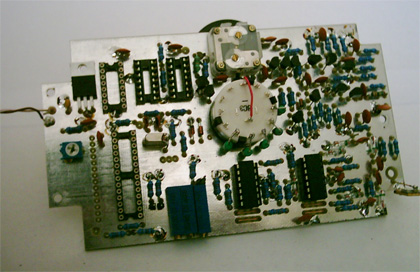
\includegraphics[width=0.8\textwidth]{obr/rozsirenie.jpg}
      \end{center}
    \end{column}
    \begin{column}{0.4\textwidth}
    \begin{block}{Možnosti rozšírenia}
    \begin{itemize}
         \item Gyrosenzor
         \item Meranie iných analógových veličín
	\end{itemize}
  \end{block}
        \end{column}
  \end{columns}
\end{snimka}